\renewcommand{\theequation}{\theenumi}
\begin{enumerate}[label=\arabic*.,ref=\thesubsection.\theenumi]
\numberwithin{equation}{enumi}
\item probability of having two girls in a family
\begin{align}
&= \frac{\text {Favourable cases} }{\text {total cases}}
\\
&=\frac{\text {No. of families having 2 girls} }{\text {total No. of families}}
\end{align} 
\\
Let assume that the probability of chosen family will have 2 girls  be $P\left(A\right)$ so 
\begin{align}
P\left(A\right)&= \frac{475}{1500}
\\
&= 0.316
\end{align}
\\
\item probability of having one  girl in a family
\begin{align}
&=\frac{\text {No. of families having 1 girl} }{\text {total No. of families}}
\end{align} 
\\
Let assume that the probability of chosen family will have 1 girl  be $P\left(B\right)$ so 
\begin{align}
P\left(B\right)&= \frac{814}{1500}
\\
&= 0.5427
\end{align} 
\\
\item probability of having one  girl in a family
\begin{align}
&=\frac{\text {No. of families having no girl} }{\text {total No. of families}}
\end{align} 
\\
Let assume that the probability of chosen family will have no girl  be $P\left(C\right)$ so 
\begin{align}
P\left(C\right)&= \frac{211}{1500}
\\
&= 0.1407
\end{align} 

\begin{align}
P(A) + P(B) + P(C) &= 0.316 + 0.5427 + 0.1407
\\
&= 1
\end{align}
codes for the above equation can be get from here
\begin{lstlisting}
codes/prob/prob2.py
\end{lstlisting}
\begin{figure}[!ht]
	\centering
	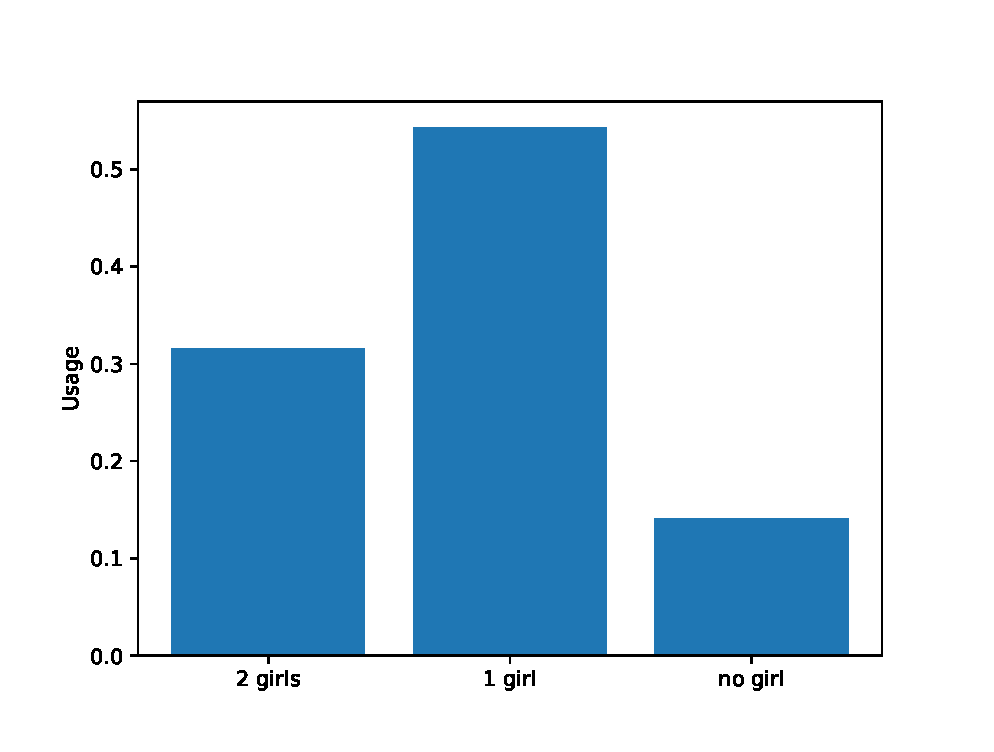
\includegraphics[width=\columnwidth]{./figures/prob/prob2.eps}
	\caption{probability 2 }
	\label{fig:bt2}
	\begin{lstlisting}
	figs/prob/prob2.py
	\end{lstlisting}
\end{figure}
\end{enumerate}